% Figures for Examined Design. Each \Fig... macro draws one figure body (no float).
\usetikzlibrary{positioning,arrows.meta,calc,shapes.misc,fit,backgrounds,decorations.pathreplacing}
\definecolor{accent}{HTML}{B4500E}
\definecolor{ok}{HTML}{2F7D4F}
\definecolor{bad}{HTML}{B3261E}
\definecolor{line}{gray}{0.35}
\definecolor{soft}{gray}{0.93}
\tikzset{
  every picture/.style={line width=0.6pt, >={Stealth[length=2.2mm]}},
  box/.style={draw=line, rounded corners=2pt, align=center, inner sep=4pt, font=\small},
  hot/.style={box, draw=accent, fill=accent!7},
  note/.style={font=\footnotesize, align=center, text=black!75},
  tiny/.style={font=\scriptsize, align=center, text=black!70},
  flow/.style={->, draw=line},
}

% ---- Prologue: two lines of testimony -------------------------------------------------
\newcommand{\FigTwoLines}{%
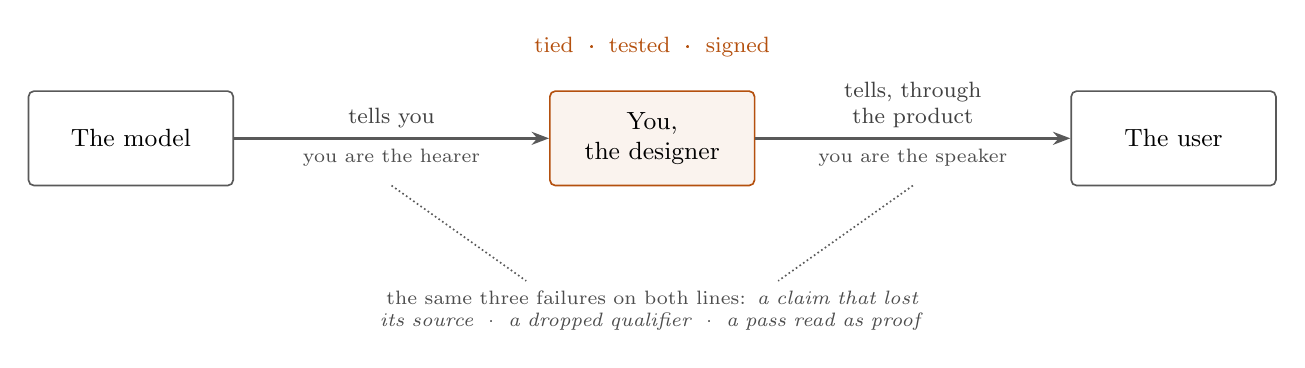
\begin{tikzpicture}
  \node[box, minimum width=26mm, minimum height=12mm] (m) {The model};
  \node[hot, minimum width=26mm, minimum height=12mm, right=40mm of m] (d) {You,\\the designer};
  \node[box, minimum width=26mm, minimum height=12mm, right=40mm of d] (u) {The user};
  \draw[flow, line width=1pt] (m) -- node[above, note]{tells you} node[below, tiny]{you are the hearer} (d);
  \draw[flow, line width=1pt] (d) -- node[above, note, align=center]{tells, through\\the product} node[below, tiny]{you are the speaker} (u);
  \node[note, above=3mm of d, text=accent] {tied \;·\; tested \;·\; signed};
  \node[tiny, below=12mm of d, text width=120mm] (f)
    {the same three failures on both lines: \textit{a claim that lost its source} \;·\; \textit{a dropped qualifier} \;·\; \textit{a pass read as proof}};
  \draw[line, densely dotted] ($(m.east)!0.5!(d.west)+(0,-6mm)$) -- ($(f.north)+(-16mm,0)$);
  \draw[line, densely dotted] ($(d.east)!0.5!(u.west)+(0,-6mm)$) -- ($(f.north)+(16mm,0)$);
\end{tikzpicture}}

% ---- Prologue: the article and the three conditions ------------------------------------
\newcommand{\FigArticleShape}{%
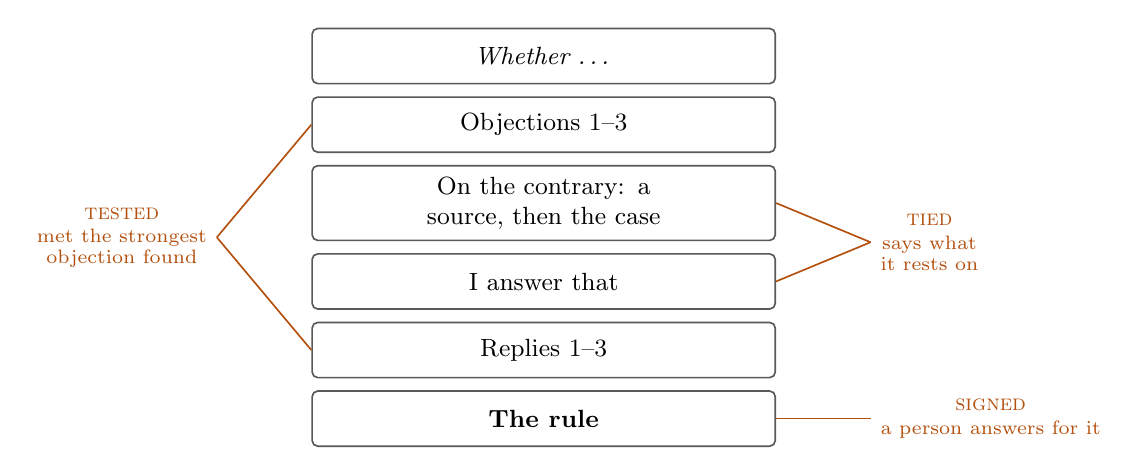
\begin{tikzpicture}[row/.style={box, text width=56mm, minimum height=7mm}]
  \node[row] (q) at (0,0) {\textit{Whether \dots}};
  \node[row, below=1.5mm of q] (o) {Objections 1--3};
  \node[row, below=1.5mm of o] (s) {On the contrary: a source, then the case};
  \node[row, below=1.5mm of s] (a) {I answer that};
  \node[row, below=1.5mm of a] (r) {Replies 1--3};
  \node[row, below=1.5mm of r, font=\small\bfseries] (b) {The rule};
  \node[note, text=accent, anchor=east] (te) at ($(o.west)!0.5!(r.west)+(-12mm,0)$) {\textsc{tested}\\[-1pt]\scriptsize met the strongest\\[-2pt]\scriptsize objection found};
  \draw[accent] (te.east) -- (o.west); \draw[accent] (te.east) -- (r.west);
  \node[note, text=accent, anchor=west] (ti) at ($(s.east)!0.5!(a.east)+(12mm,0)$) {\textsc{tied}\\[-1pt]\scriptsize says what\\[-2pt]\scriptsize it rests on};
  \draw[accent] (ti.west) -- (s.east); \draw[accent] (ti.west) -- (a.east);
  \node[note, text=accent, anchor=west] (si) at ($(b.east)+(12mm,0)$) {\textsc{signed}\\[-1pt]\scriptsize a person answers for it};
  \draw[accent] (si.west) -- (b.east);
\end{tikzpicture}}

% ---- The loop: going out and coming back -------------------------------------------------
\newcommand{\FigLoop}{%
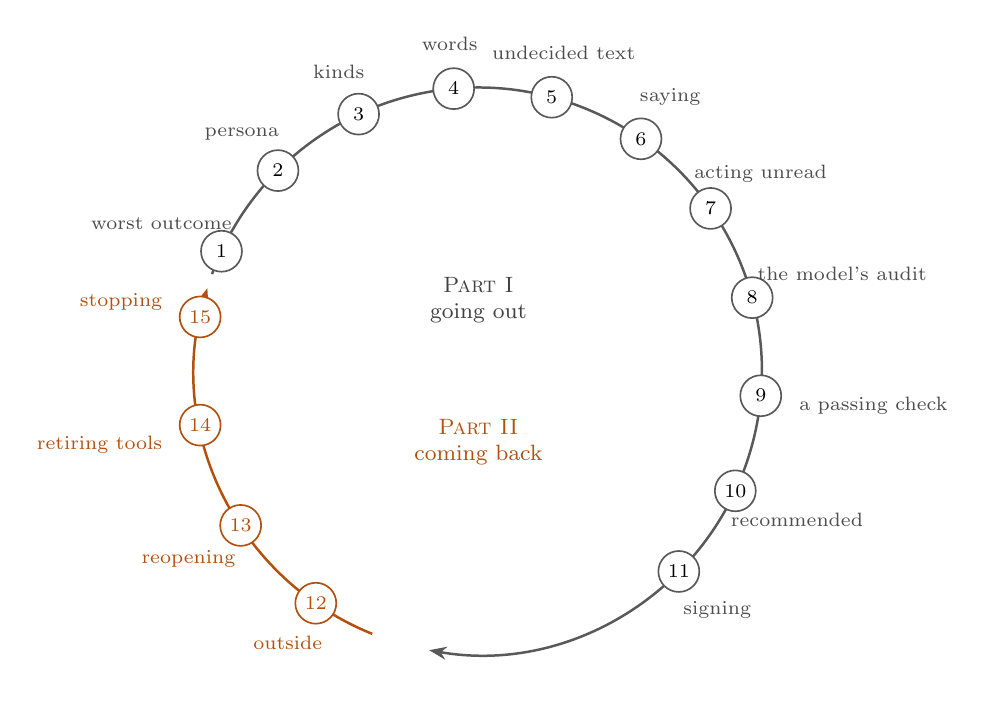
\begin{tikzpicture}
  \def\R{36mm}
  \draw[line, ->, line width=0.9pt] (160:\R) arc[start angle=160, end angle=-100, radius=\R];
  \draw[accent, ->, line width=0.9pt] (-112:\R) arc[start angle=-112, end angle=-197, radius=\R];
  \foreach \n/\a/\t in {1/155/worst outcome,2/135/persona,3/115/kinds,4/95/words,5/75/undecided text,6/55/saying,7/35/acting unread,8/15/the model's audit,9/-5/a passing check,10/-25/recommended,11/-45/signing}{
    \node[circle, draw=line, fill=white, inner sep=1.2pt, minimum size=5.2mm, font=\scriptsize] at (\a:\R) {\n};
    \node[tiny, anchor={\a+180}] at (\a:\R+3.6mm) {\t};
  }
  \foreach \n/\a/\t in {12/-125/outside,13/-147/reopening,14/-169/retiring tools,15/-191/stopping}{
    \node[circle, draw=accent, fill=white, inner sep=1.2pt, minimum size=5.2mm, font=\scriptsize, text=accent] at (\a:\R) {\n};
    \node[tiny, anchor={\a+180}, text=accent] at (\a:\R+3.6mm) {\t};
  }
  \node[note] at (0,9mm) {\textsc{Part I}\\going out};
  \node[note, text=accent] at (0,-9mm) {\textsc{Part II}\\coming back};
\end{tikzpicture}}

% ---- Article 1: what makes an outcome the worst ------------------------------------------
\newcommand{\FigWorst}{%
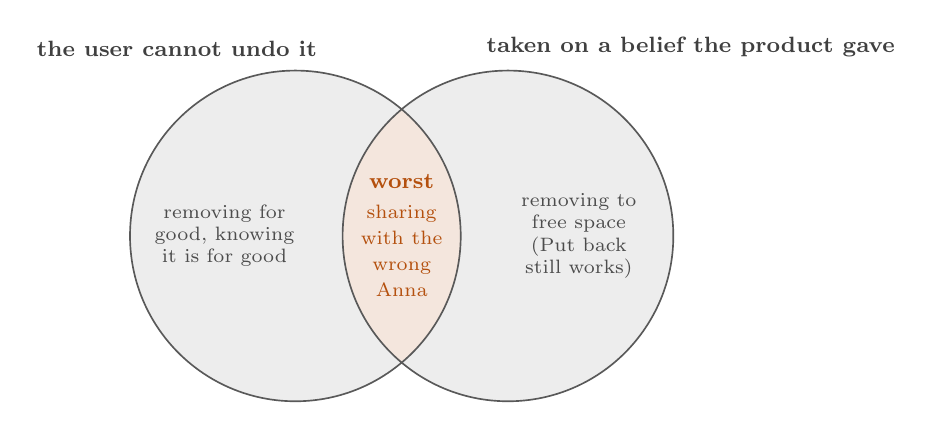
\begin{tikzpicture}
  \fill[soft] (0,0) circle (21mm);
  \fill[soft] (27mm,0) circle (21mm);
  \begin{scope}
    \clip (0,0) circle (21mm);
    \fill[accent!14] (27mm,0) circle (21mm);
  \end{scope}
  \draw[line] (0,0) circle (21mm) (27mm,0) circle (21mm);
  \node[note, font=\footnotesize\bfseries, anchor=south east] at (4mm,21.5mm) {the user cannot undo it};
  \node[note, font=\footnotesize\bfseries, anchor=south west] at (23mm,21.5mm) {taken on a belief the product gave};
  \node[tiny, text width=19mm] at (-9mm,0) {removing for good, knowing it is for good};
  \node[tiny, text width=19mm] at (36mm,0) {removing to free space (Put back still works)};
  \node[note, text width=13mm, text=accent] at (13.5mm,0) {\textbf{worst}\\[1pt]\scriptsize sharing with the wrong Anna};
\end{tikzpicture}}

% ---- Article 2: a yardstick, a check, and the remainder ----------------------------------
\newcommand{\FigYardstick}{%
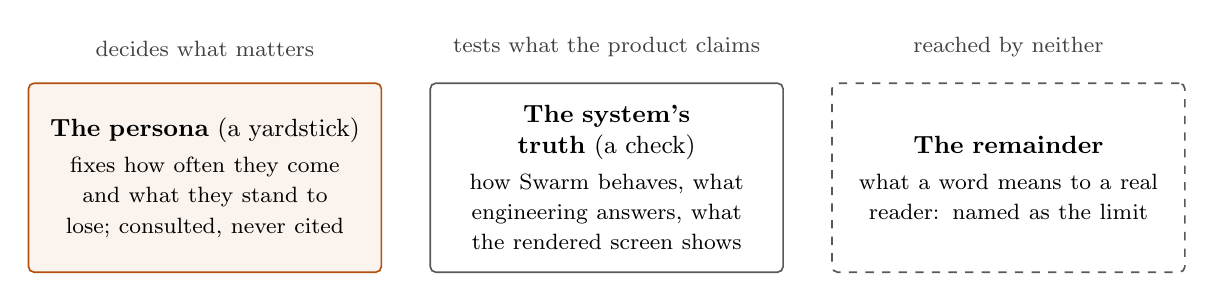
\begin{tikzpicture}
  \node[hot, text width=42mm, minimum height=24mm] (p) {\textbf{The persona} (a yardstick)\\[2pt]\footnotesize fixes how often they come and what they stand to lose; consulted, never cited};
  \node[box, text width=42mm, minimum height=24mm, right=6mm of p] (s) {\textbf{The system's truth} (a check)\\[2pt]\footnotesize how Swarm behaves, what engineering answers, what the rendered screen shows};
  \node[box, dashed, text width=42mm, minimum height=24mm, right=6mm of s] (r) {\textbf{The remainder}\\[2pt]\footnotesize what a word means to a real reader: named as the limit};
  \node[note, above=2mm of p] {decides what matters};
  \node[note, above=2mm of s] {tests what the product claims};
  \node[note, above=2mm of r] {reached by neither};
\end{tikzpicture}}

% ---- Article 3: a kind earns its place by an obligation ----------------------------------
\newcommand{\FigKinds}{%
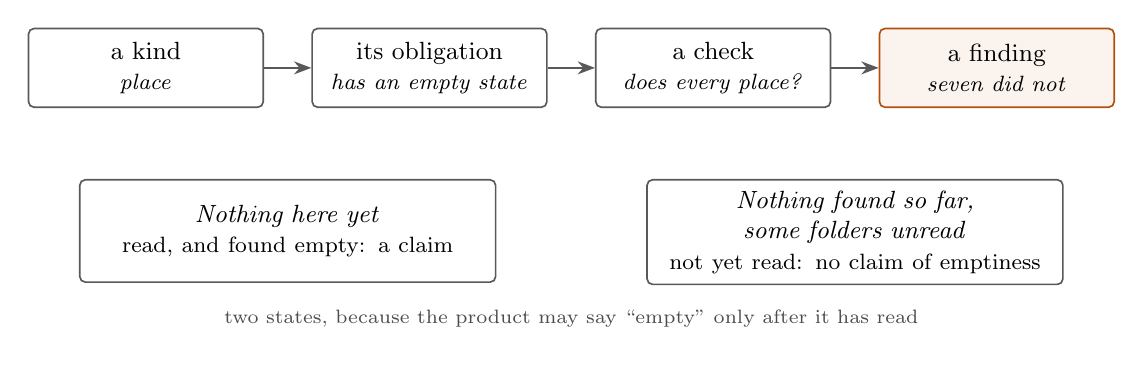
\begin{tikzpicture}[st/.style={box, minimum height=10mm, text width=27mm}]
  \node[st] (k) {a kind\\\footnotesize\textit{place}};
  \node[st, right=6mm of k] (o) {its obligation\\\footnotesize\textit{has an empty state}};
  \node[st, right=6mm of o] (c) {a check\\\footnotesize\textit{does every place?}};
  \node[hot, minimum height=10mm, text width=27mm, right=6mm of c] (f) {a finding\\\footnotesize\textit{seven did not}};
  \draw[flow] (k) -- (o); \draw[flow] (o) -- (c); \draw[flow] (c) -- (f);
  \node[box, text width=50mm, minimum height=13mm, anchor=north] (e) at ($(k.south)!0.5!(o.south)+(0,-9mm)$) {\textit{Nothing here yet}\\\footnotesize read, and found empty: a claim};
  \node[box, text width=50mm, minimum height=13mm, anchor=north] (n) at ($(c.south)!0.5!(f.south)+(0,-9mm)$) {\textit{Nothing found so far, some folders unread}\\\footnotesize not yet read: no claim of emptiness};
  \node[tiny, anchor=north] at ($(e.south)!0.5!(n.south)+(0,-2mm)$) {two states, because the product may say ``empty'' only after it has read};
\end{tikzpicture}}

% ---- Article 4: the implicature check ------------------------------------------------------
\newcommand{\FigImplicature}{%
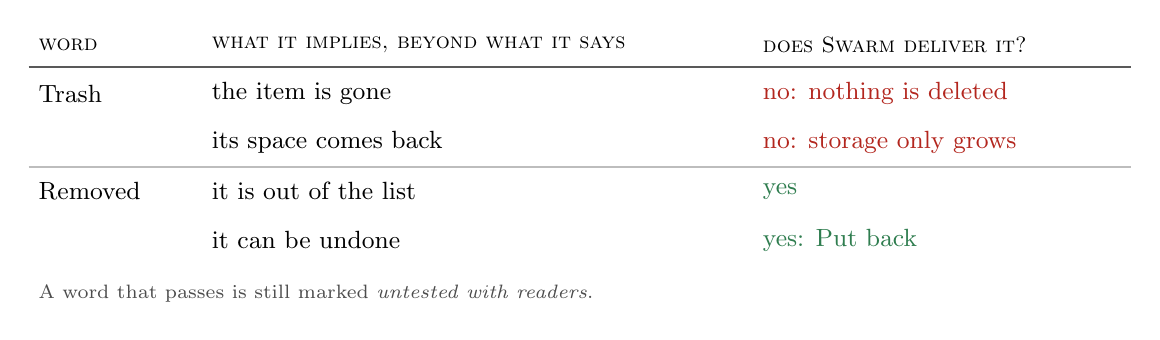
\begin{tikzpicture}[c/.style={font=\small, anchor=west}, y=6.2mm]
  \node[c, font=\footnotesize\scshape] at (0,0) {word};
  \node[c, font=\footnotesize\scshape] at (22mm,0) {what it implies, beyond what it says};
  \node[c, font=\footnotesize\scshape] at (92mm,0) {does Swarm deliver it?};
  \draw[line] (0,-0.45) -- (140mm,-0.45);
  \node[c] at (0,-1) {Trash}; \node[c] at (22mm,-1) {the item is gone}; \node[c, text=bad] at (92mm,-1) {no: nothing is deleted};
  \node[c] at (22mm,-2) {its space comes back}; \node[c, text=bad] at (92mm,-2) {no: storage only grows};
  \draw[line!40] (0,-2.5) -- (140mm,-2.5);
  \node[c] at (0,-3) {Removed}; \node[c] at (22mm,-3) {it is out of the list}; \node[c, text=ok] at (92mm,-3) {yes};
  \node[c] at (22mm,-4) {it can be undone}; \node[c, text=ok] at (92mm,-4) {yes: Put back};
  \node[tiny, anchor=west] at (0,-5.1) {A word that passes is still marked \textit{untested with readers}.};
\end{tikzpicture}}

% ---- Article 5: where undecided text may go -----------------------------------------------
\newcommand{\FigTextPath}{%
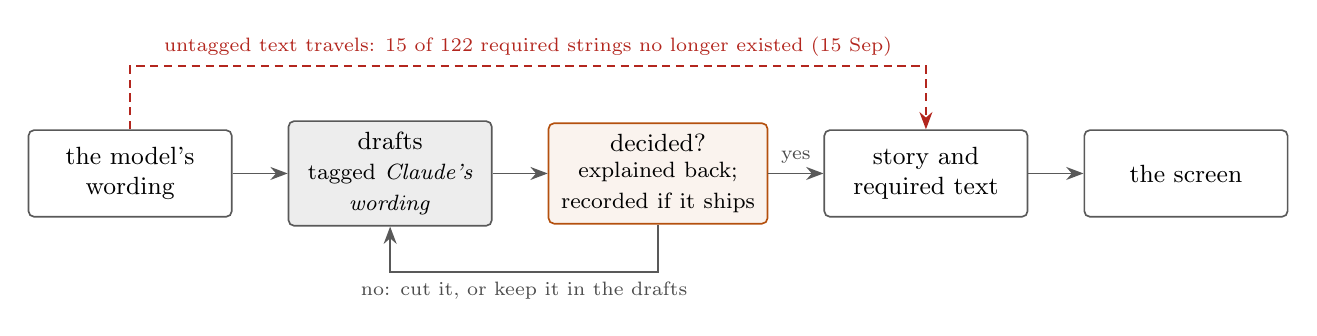
\begin{tikzpicture}[st/.style={box, minimum height=11mm, text width=23mm}]
  \node[st] (m) {the model's\\wording};
  \node[st, right=7mm of m, fill=soft] (d) {drafts\\\footnotesize tagged \textit{Claude's wording}};
  \node[hot, minimum height=11mm, text width=25mm, right=7mm of d] (g) {decided?\\\footnotesize explained back;\\recorded if it ships};
  \node[st, right=7mm of g] (s) {story and\\required text};
  \node[st, right=7mm of s] (u) {the screen};
  \draw[flow] (m) -- (d); \draw[flow] (d) -- (g); \draw[flow] (g) -- node[above, tiny]{yes} (s); \draw[flow] (s) -- (u);
  \draw[flow] (g.south) -- ++(0,-6mm) -| node[pos=0.25, below, tiny]{no: cut it, or keep it in the drafts} (d.south);
  \draw[->, bad, densely dashed] (m.north) -- ++(0,8mm) -| node[pos=0.25, above, tiny, text=bad]{untagged text travels: 15 of 122 required strings no longer existed (15 Sep)} (s.north);
\end{tikzpicture}}

% ---- Article 6: what was observed, and how far it reaches ----------------------------------
\newcommand{\FigObserved}{%
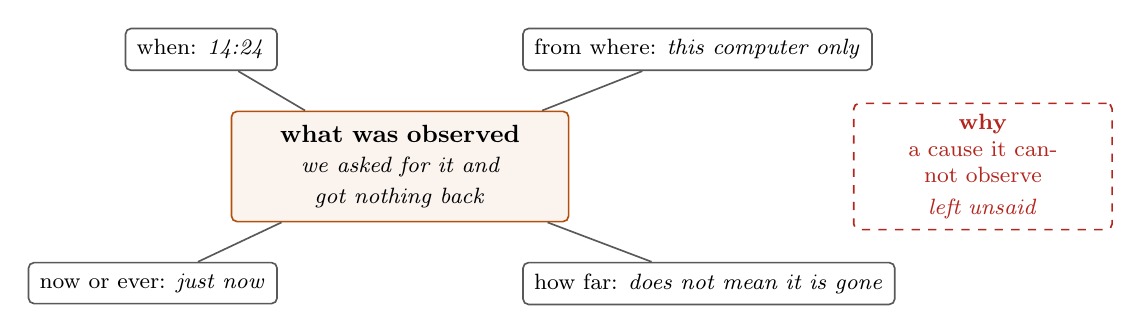
\begin{tikzpicture}
  \node[hot, text width=40mm, minimum height=14mm] (o) {\textbf{what was observed}\\\footnotesize\textit{we asked for it and got nothing back}};
  \node[box, above left=5mm and -6mm of o, font=\footnotesize] (w) {when: \textit{14:24}};
  \node[box, above right=5mm and -6mm of o, font=\footnotesize] (f) {from where: \textit{this computer only}};
  \node[box, below left=5mm and -6mm of o, font=\footnotesize] (n) {now or ever: \textit{just now}};
  \node[box, below right=5mm and -6mm of o, font=\footnotesize] (h) {how far: \textit{does not mean it is gone}};
  \foreach \x in {w,f,n,h} \draw[line] (o) -- (\x);
  \node[box, dashed, draw=bad, right=36mm of o, text width=30mm, font=\footnotesize, text=bad] (y) {\textbf{why}\\a cause it cannot observe\\[2pt]\textit{left unsaid}};
\end{tikzpicture}}

% ---- Article 7: the life of a read ---------------------------------------------------------
\newcommand{\FigRead}{%
\begin{tikzpicture}[seg/.style={box, minimum height=17mm, font=\footnotesize, text width=##1}, x=1mm]
  \node[seg=19mm, fill=white] (a) at (0,0) {a short pause\\\textit{nothing shown}};
  \node[seg=27mm, fill=soft, right=0mm of a] (b) {placeholders\\\textit{``Reading your list\dots''}};
  \node[seg=27mm, fill=soft, right=0mm of b] (c) {if it runs long\\\textit{``taking longer than usual''}};
  \node[box, draw=ok, minimum height=8mm, text width=40mm, font=\footnotesize, right=7mm of c, yshift=7mm] (r) {read: figures and badges shown};
  \node[box, draw=bad, minimum height=8mm, text width=40mm, font=\footnotesize, right=7mm of c, yshift=-7mm] (x) {failed: last read kept, \textit{with its time}; Try again};
  \draw[flow] (c.east) -- (r.west); \draw[flow] (c.east) -- (x.west);
  \draw[line, ->] ($(a.north west)+(0,4mm)$) -- node[above, tiny, pos=0.5]{time} ($(c.north east)+(0,4mm)$);
  \node[font=\footnotesize, anchor=east] at ($(a.south west)+(-2mm,-6mm)$) {commit};
  \draw[bad, line width=2pt] ($(a.south west)+(0,-6mm)$) -- ($(c.south east)+(0,-6mm)$);
  \node[tiny, text=bad, anchor=north] at ($(b.south)!0.5!(c.south)+(0,-7mm)$) {off until its facts are read};
  \node[font=\footnotesize, anchor=east] at ($(a.south west)+(-2mm,-13mm)$) {cancel};
  \draw[ok, line width=2pt] ($(a.south west)+(0,-13mm)$) -- ($(x.east |- a.south)+(0,-13mm)$);
  \node[tiny, text=ok, anchor=north] at ($(b.south)!0.5!(c.south)+(0,-14mm)$) {always works};
  \node[tiny, text=ok, anchor=west] at ($(r.east)+(1mm,0)$) {commit on};
  \node[tiny, text=bad, anchor=west] at ($(x.east)+(1mm,0)$) {commit off};
\end{tikzpicture}}

% ---- Charts redrawn from studies (numbers exactly as in research/*.md) --------------------
\pgfplotsset{compat=1.18,
  every axis/.append style={font=\scriptsize, axis line style={line}, tick style={line}, label style={font=\footnotesize}},
}

% Article 3: Nielsen (1994), cumulative variance explained by factors (text of the paper).
\newcommand{\ChartNielsen}{%
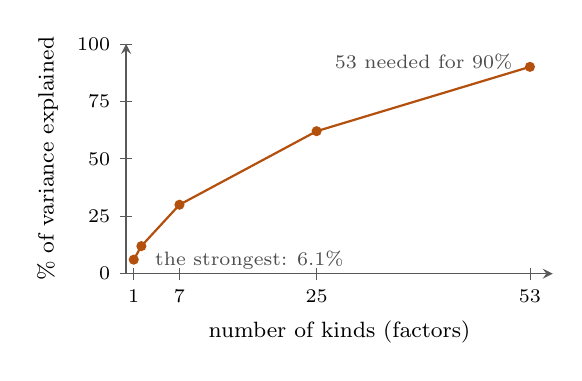
\begin{tikzpicture}
\begin{axis}[width=70mm, height=45mm, xmin=0, xmax=56, ymin=0, ymax=100,
  xlabel={number of kinds (factors)}, ylabel={\% of variance explained},
  xtick={1,7,25,53}, ytick={0,25,50,75,100}, axis lines=left, clip=false]
  \addplot[accent, mark=*, mark size=1.4pt, line width=0.8pt] coordinates {(1,6.1) (2,12.0) (7,30) (25,62) (53,90)};
  \node[tiny, anchor=west] at (axis cs:2.5,6) {the strongest: 6.1\%};
  \node[tiny, anchor=east] at (axis cs:52,92) {53 needed for 90\%};
\end{axis}
\end{tikzpicture}}

% Article 4: Doshi & Hauser (2024), Figs 2 and 4; effects of one / five AI ideas.
\newcommand{\ChartDoshi}{%
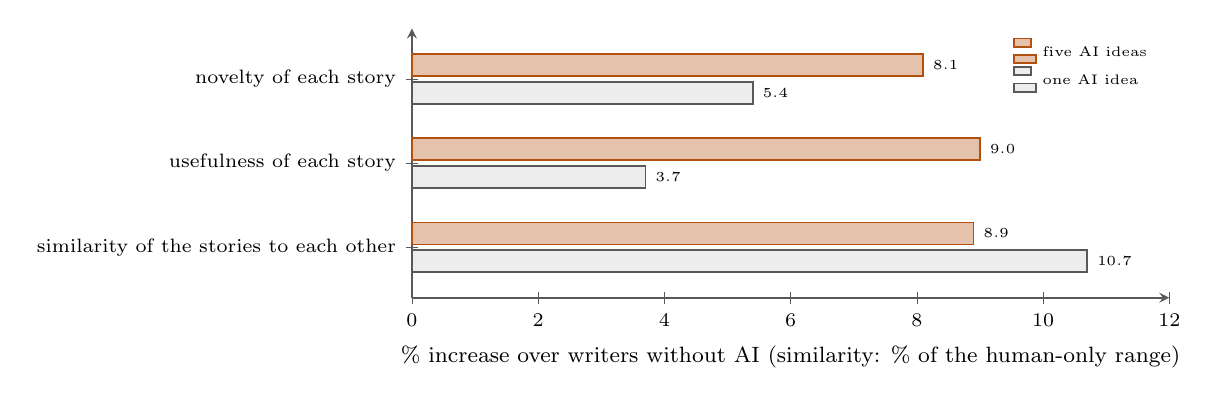
\begin{tikzpicture}
\begin{axis}[width=112mm, height=50mm, xbar, bar width=2.8mm, xmin=0, xmax=12, clip=false,
  ymin=-0.6, ymax=2.6, ytick={0,1,2}, yticklabels={similarity of the stories to each other,usefulness of each story,novelty of each story}, xlabel={\% increase over writers without AI (similarity: \% of the human-only range)}, axis lines=left,
  nodes near coords, every node near coord/.append style={font=\tiny, /pgf/number format/fixed, /pgf/number format/precision=1, /pgf/number format/fixed zerofill},
  legend style={font=\tiny, draw=none, at={(0.99,0.99)}, anchor=north east}, legend cell align=left, reverse legend]
  \addplot[fill=soft, draw=line] coordinates {(10.7,0) (3.7,1) (5.4,2)};
  \addplot[fill=accent!35, draw=accent] coordinates {(8.9,0) (9.0,1) (8.1,2)};
  \legend{one AI idea, five AI ideas}
\end{axis}
\end{tikzpicture}}

% Article 6: van der Bles et al. (2020), Fig. 5, internal meta-analysis of experiments 1-4 (Cohen's d).
\newcommand{\ChartVanDerBles}{%
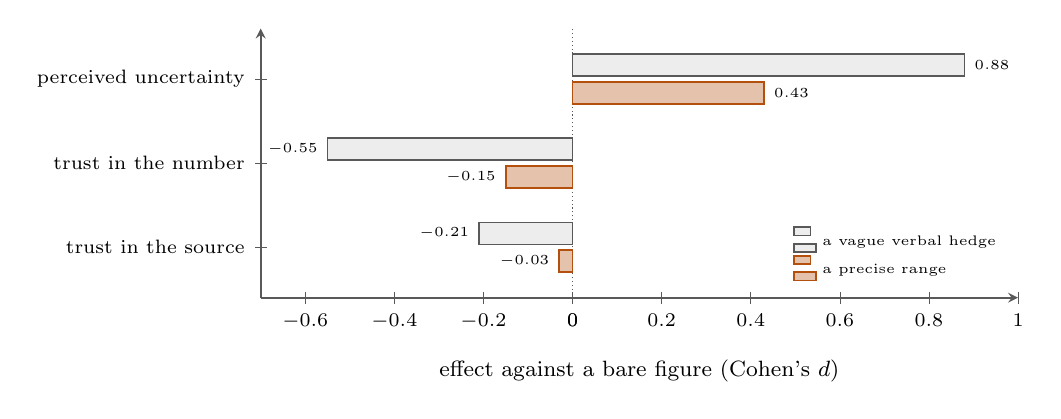
\begin{tikzpicture}
\begin{axis}[width=112mm, height=50mm, xbar, bar width=2.8mm, xmin=-0.7, xmax=1.0, clip=false,
  ymin=-0.6, ymax=2.6, ytick={0,1,2}, yticklabels={trust in the source,trust in the number,perceived uncertainty}, xlabel={effect against a bare figure (Cohen's $d$)}, axis lines=left,
  extra x ticks={0}, extra x tick style={grid=major, grid style={line, densely dotted}},
  nodes near coords, every node near coord/.append style={font=\tiny, /pgf/number format/fixed, /pgf/number format/precision=2, /pgf/number format/fixed zerofill},
  legend style={font=\tiny, draw=none, at={(0.99,0.03)}, anchor=south east}, legend cell align=left, reverse legend]
  \addplot[fill=accent!35, draw=accent] coordinates {(-0.03,0) (-0.15,1) (0.43,2)};
  \addplot[fill=soft, draw=line] coordinates {(-0.21,0) (-0.55,1) (0.88,2)};
  \legend{a precise range, a vague verbal hedge}
\end{axis}
\end{tikzpicture}}

% ---- Article 8: slices, a merge, and what the circle threatens ------------------------------
\newcommand{\FigAudit}{%
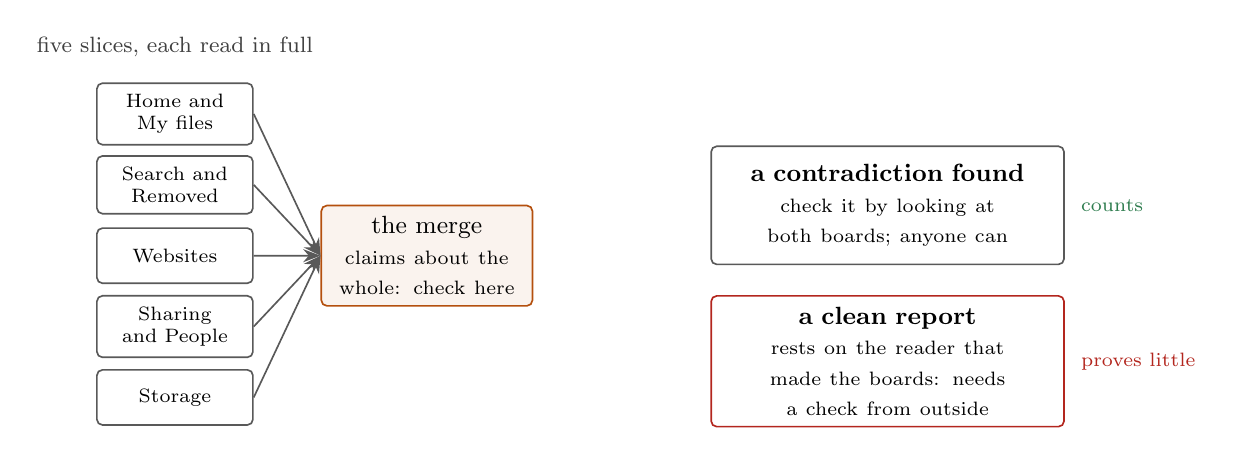
\begin{tikzpicture}[sl/.style={box, minimum width=17mm, minimum height=7mm, font=\scriptsize}]
  \foreach \i/\t in {0/Home and My files,1/Search and Removed,2/Websites,3/Sharing and People,4/Storage}{
    \node[sl, text width=17mm] (s\i) at (0,-\i*9mm) {\t};
  }
  \node[hot, text width=24mm, minimum height=12mm] (mg) at (32mm,-18mm) {the merge\\\scriptsize claims about the whole: check here};
  \foreach \i in {0,...,4} \draw[flow] (s\i.east) -- (mg.west);
  \node[note, above=2mm of s0] {five slices, each read in full};
  \begin{scope}[xshift=68mm, yshift=-4mm]
    \node[box, text width=42mm, minimum height=15mm, anchor=north west] (f) at (0,0) {\textbf{a contradiction found}\\\scriptsize check it by looking at both boards; anyone can};
    \node[box, draw=bad, text width=42mm, minimum height=15mm, anchor=north west] (c) at (0,-19mm) {\textbf{a clean report}\\\scriptsize rests on the reader that made the boards: needs a check from outside};
    \node[tiny, text=ok, anchor=west] at (f.east) {\;counts};
    \node[tiny, text=bad, anchor=west] at (c.east) {\;proves little};
  \end{scope}
\end{tikzpicture}}

% Article 8: Liu et al. (2024), arXiv v3 Table 6; gpt-3.5-turbo-0613, 20 documents.
\newcommand{\ChartLiu}{%
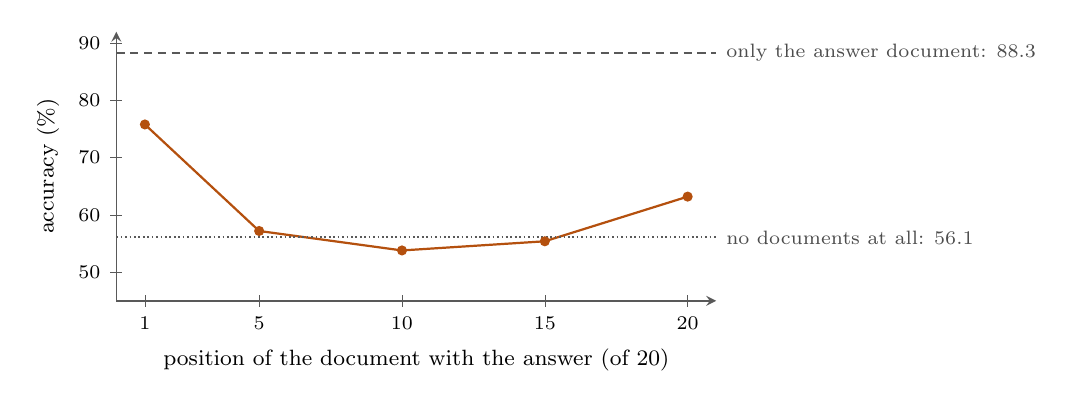
\begin{tikzpicture}
\begin{axis}[width=92mm, height=50mm, xmin=0, xmax=21, ymin=45, ymax=92, axis lines=left,
  xtick={1,5,10,15,20}, ytick={50,60,70,80,90}, xlabel={position of the document with the answer (of 20)}, ylabel={accuracy (\%)}, clip=false]
  \addplot[accent, mark=*, mark size=1.4pt, line width=0.8pt] coordinates {(1,75.8) (5,57.2) (10,53.8) (15,55.4) (20,63.2)};
  \draw[line, densely dashed] (axis cs:0,88.3) -- (axis cs:21,88.3) node[tiny, anchor=west]{only the answer document: 88.3};
  \draw[line, densely dotted] (axis cs:0,56.1) -- (axis cs:21,56.1) node[tiny, anchor=west]{no documents at all: 56.1};
\end{axis}
\end{tikzpicture}}

% ---- Article 9: the veil (project data) and what each check cannot see -----------------------
\newcommand{\ChartVeil}{%
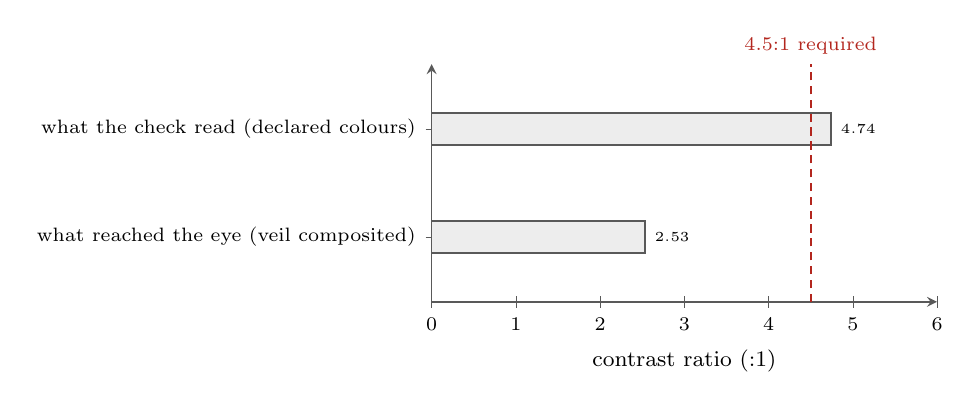
\begin{tikzpicture}
\begin{axis}[width=80mm, height=46mm, xbar, bar width=4mm, xmin=0, xmax=6, clip=false,
  ymin=-0.6, ymax=1.6, ytick={0,1}, yticklabels={what reached the eye (veil composited),what the check read (declared colours)},
  xlabel={contrast ratio (:1)}, axis lines=left, nodes near coords, every node near coord/.append style={font=\tiny, /pgf/number format/fixed, /pgf/number format/precision=2, /pgf/number format/fixed zerofill}]
  \addplot[fill=soft, draw=line] coordinates {(2.53,0) (4.74,1)};
  \draw[bad, densely dashed] (axis cs:4.5,-0.6) -- (axis cs:4.5,1.6) node[tiny, text=bad, anchor=south]{4.5:1 required};
\end{axis}
\end{tikzpicture}}

\newcommand{\FigCannotSee}{%
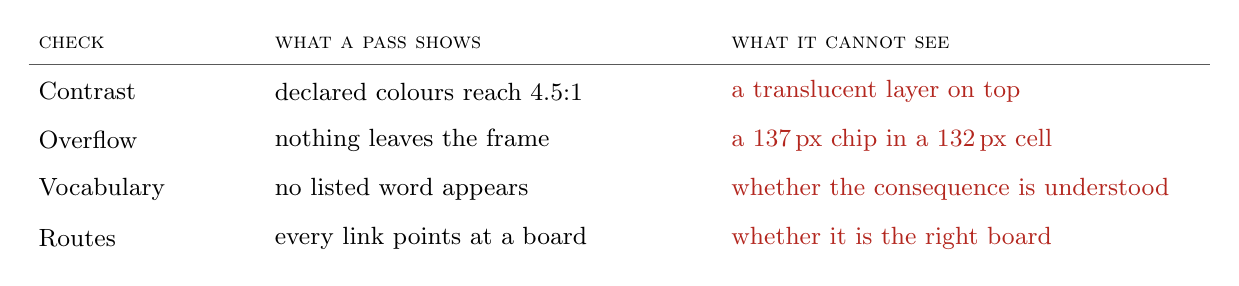
\begin{tikzpicture}[c/.style={font=\small, anchor=west}, y=6.2mm]
  \node[c, font=\footnotesize\scshape] at (0,0) {check}; \node[c, font=\footnotesize\scshape] at (30mm,0) {what a pass shows}; \node[c, font=\footnotesize\scshape] at (88mm,0) {what it cannot see};
  \draw[line] (0,-0.45) -- (150mm,-0.45);
  \node[c] at (0,-1) {Contrast}; \node[c] at (30mm,-1) {declared colours reach 4.5:1}; \node[c, text=bad] at (88mm,-1) {a translucent layer on top};
  \node[c] at (0,-2) {Overflow}; \node[c] at (30mm,-2) {nothing leaves the frame}; \node[c, text=bad] at (88mm,-2) {a 137\,px chip in a 132\,px cell};
  \node[c] at (0,-3) {Vocabulary}; \node[c] at (30mm,-3) {no listed word appears}; \node[c, text=bad] at (88mm,-3) {whether the consequence is understood};
  \node[c] at (0,-4) {Routes}; \node[c] at (30mm,-4) {every link points at a board}; \node[c, text=bad] at (88mm,-4) {whether it is the right board};
\end{tikzpicture}}

% ---- Article 10: defaults (Johnson & Goldstein 2003, online experiment) and this paper's record --
\newcommand{\ChartDefaults}{%
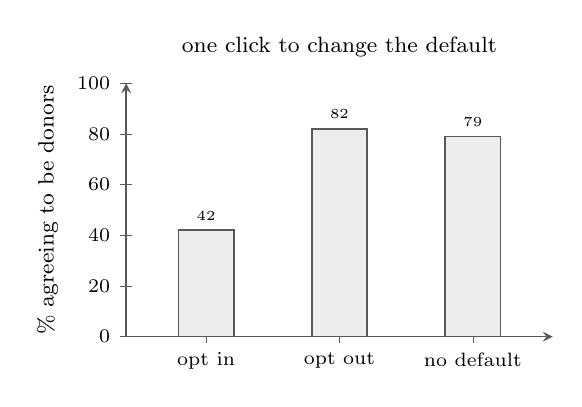
\begin{tikzpicture}
\begin{axis}[width=70mm, height=48mm, ybar, bar width=7mm, ymin=0, ymax=100, axis lines=left,
  xmin=0.4, xmax=3.6, xtick={1,2,3}, xticklabels={opt in,opt out,no default}, ylabel={\% agreeing to be donors},
  title={\footnotesize one click to change the default}, nodes near coords, every node near coord/.append style={font=\tiny}]
  \addplot[fill=soft, draw=line] coordinates {(1,42) (2,82) (3,79)};
\end{axis}
\end{tikzpicture}\hspace{6mm}%
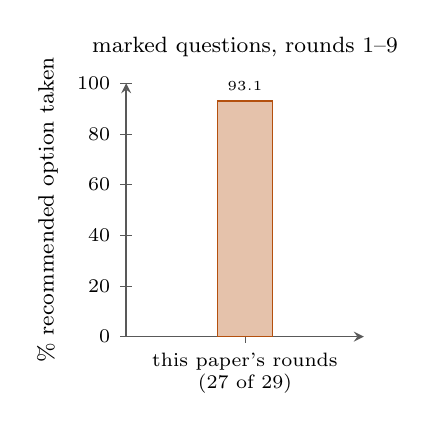
\begin{tikzpicture}
\begin{axis}[width=46mm, height=48mm, ybar, bar width=7mm, ymin=0, ymax=100, axis lines=left,
  xmin=0.4, xmax=1.6, xtick={1}, xticklabels={this paper's rounds\\(27 of 29)}, xticklabel style={align=center}, ylabel={\% recommended option taken},
  title={\footnotesize marked questions, rounds 1--9}, nodes near coords, every node near coord/.append style={font=\tiny}]
  \addplot[fill=accent!35, draw=accent] coordinates {(1,93.1)};
\end{axis}
\end{tikzpicture}}

\newcommand{\FigEcho}{%
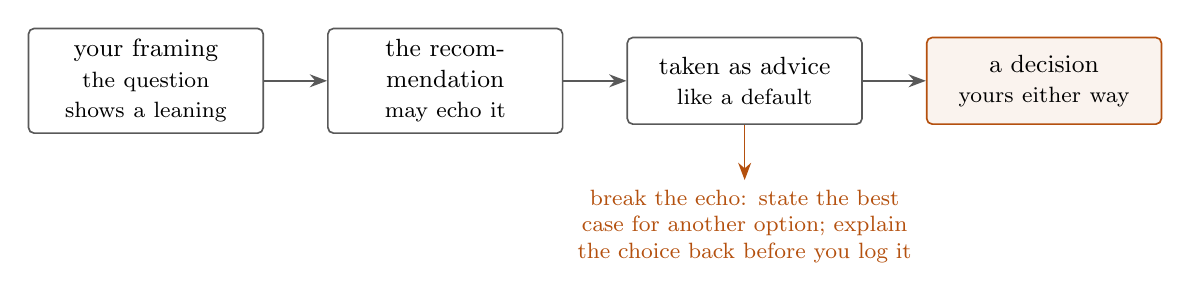
\begin{tikzpicture}[st/.style={box, minimum height=11mm, text width=27mm}]
  \node[st] (y) {your framing\\\footnotesize the question shows a leaning};
  \node[st, right=8mm of y] (m) {the recommendation\\\footnotesize may echo it};
  \node[st, right=8mm of m] (t) {taken as advice\\\footnotesize like a default};
  \node[hot, minimum height=11mm, text width=27mm, right=8mm of t] (d) {a decision\\\footnotesize yours either way};
  \draw[flow] (y) -- (m); \draw[flow] (m) -- (t); \draw[flow] (t) -- (d);
  \draw[->, accent] (t.south) -- ++(0,-7mm) node[below, note, text=accent, text width=60mm] {break the echo: state the best case for another option; explain the choice back before you log it};
\end{tikzpicture}}

% ---- Article 11: the chain from a screen to a signature ---------------------------------------
\newcommand{\FigSignChain}{%
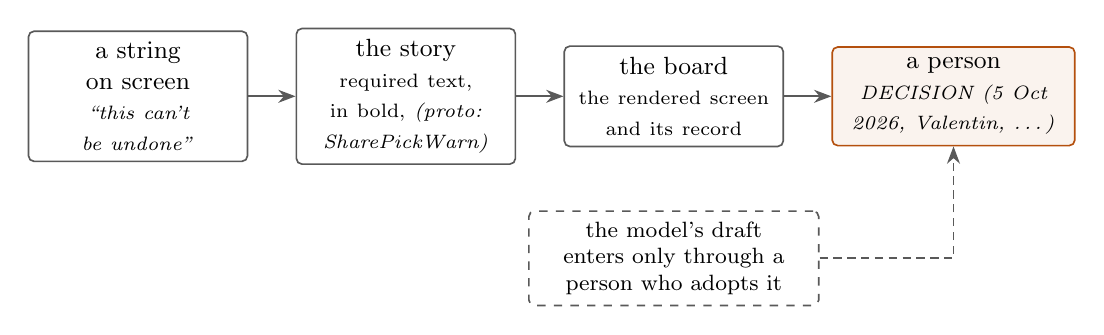
\begin{tikzpicture}[st/.style={box, minimum height=12mm, text width=25mm}]
  \node[st] (s) {a string on screen\\\scriptsize\textit{``this can't be undone''}};
  \node[st, right=6mm of s] (j) {the story\\\scriptsize required text, in bold, \textit{(proto: SharePickWarn)}};
  \node[st, right=6mm of j] (b) {the board\\\scriptsize the rendered screen and its record};
  \node[hot, minimum height=12mm, text width=28mm, right=6mm of b] (p) {a person\\\scriptsize\textit{DECISION (5 Oct 2026, Valentin, \dots)}};
  \draw[flow] (s) -- (j); \draw[flow] (j) -- (b); \draw[flow] (b) -- (p);
  \node[box, dashed, text width=34mm, font=\footnotesize, below=8mm of b] (m) {the model's draft enters only through a person who adopts it};
  \draw[flow, densely dashed] (m.east) -| (p.south);
\end{tikzpicture}}

% ---- Article 12: the circle and what lies outside it -----------------------------------------
\newcommand{\FigOutside}{%
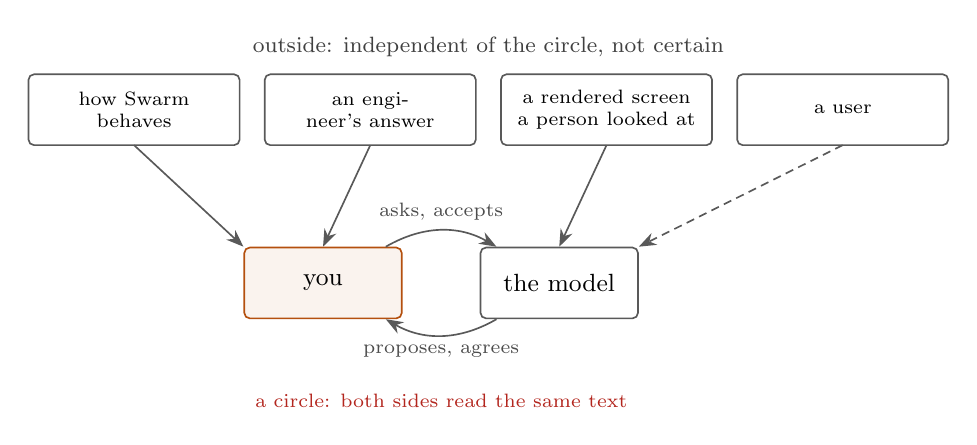
\begin{tikzpicture}
  \node[hot, minimum width=20mm, minimum height=9mm] (d) at (0,0) {you};
  \node[box, minimum width=20mm, minimum height=9mm] (m) at (30mm,0) {the model};
  \draw[flow, bend left=30] (d) to node[above, tiny]{asks, accepts} (m);
  \draw[flow, bend left=30] (m) to node[below, tiny]{proposes, agrees} (d);
  \node[tiny, text=bad] at (15mm,-15mm) {a circle: both sides read the same text};
  \foreach \t/\x in {how Swarm behaves/-24,an engineer's answer/6,a rendered screen a person looked at/36,a user/66}{
    \node[box, font=\scriptsize, text width=24mm, minimum height=9mm] (o) at (\x mm,22mm) {\t};
  }
  \draw[flow] (-24mm,17.5mm) -- (d.north west);
  \draw[flow] (6mm,17.5mm) -- (d.north);
  \draw[flow] (36mm,17.5mm) -- (m.north);
  \draw[flow, densely dashed] (66mm,17.5mm) -- (m.north east);
  \node[note] at (21mm,30mm) {outside: independent of the circle, not certain};
\end{tikzpicture}}

% Article 12: Huang et al. (2024), Tables 2-3, GPT-3.5.
\newcommand{\ChartHuang}{%
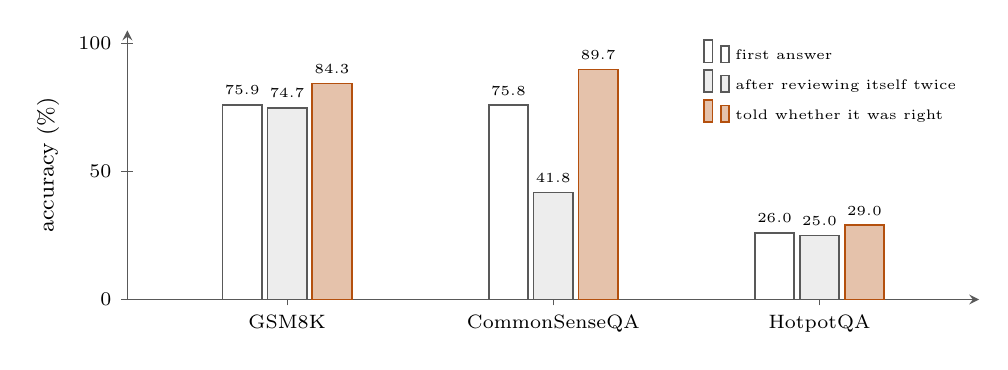
\begin{tikzpicture}
\begin{axis}[width=124mm, height=50mm, ybar=2pt, bar width=5mm, ymin=0, ymax=105, axis lines=left,
  xmin=0.4, xmax=3.6, xtick={1,2,3}, xticklabels={GSM8K,CommonSenseQA,HotpotQA}, ylabel={accuracy (\%)},
  nodes near coords, every node near coord/.append style={font=\tiny, /pgf/number format/fixed, /pgf/number format/precision=1, /pgf/number format/fixed zerofill},
  legend style={font=\tiny, draw=none, at={(0.99,0.99)}, anchor=north east}, legend cell align=left]
  \addplot[fill=white, draw=line] coordinates {(1,75.9) (2,75.8) (3,26.0)};
  \addplot[fill=soft, draw=line] coordinates {(1,74.7) (2,41.8) (3,25.0)};
  \addplot[fill=accent!35, draw=accent] coordinates {(1,84.3) (2,89.7) (3,29.0)};
  \legend{first answer, after reviewing itself twice, told whether it was right}
\end{axis}
\end{tikzpicture}}

% ---- Article 13: when to reopen -----------------------------------------------------------------
\newcommand{\FigReopen}{%
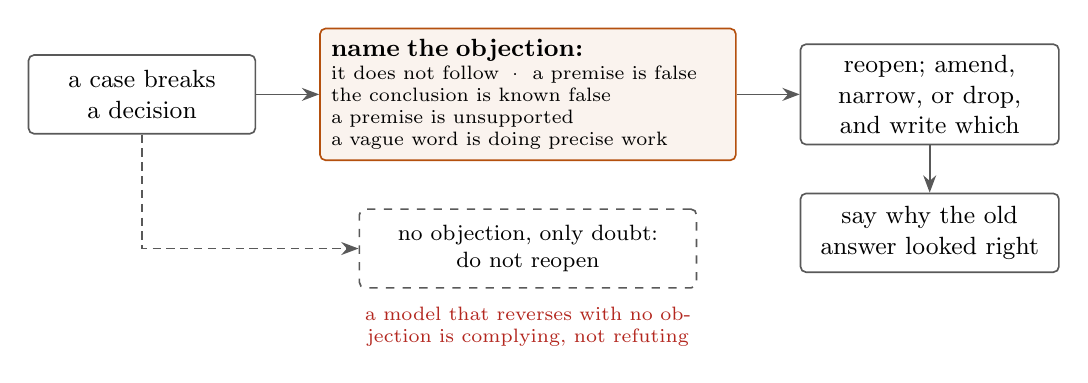
\begin{tikzpicture}[st/.style={box, minimum height=10mm}]
  \node[st, text width=26mm] (c) {a case breaks a decision};
  \node[hot, text width=50mm, right=8mm of c, align=left, font=\scriptsize] (o) {\textbf{\small name the objection:}\\
    it does not follow \;·\; a premise is false\\the conclusion is known false\\a premise is unsupported\\a vague word is doing precise work};
  \node[st, text width=30mm, right=8mm of o] (r) {reopen; amend, narrow, or drop, and write which};
  \node[st, text width=30mm, below=6mm of r] (e) {say why the old answer looked right};
  \draw[flow] (c) -- (o); \draw[flow] (o) -- (r); \draw[flow] (r) -- (e);
  \node[st, dashed, text width=40mm, below=6mm of o, font=\footnotesize] (n) {no objection, only doubt: \\do not reopen};
  \draw[flow, densely dashed] (c.south) |- (n.west);
  \node[tiny, text=bad, below=1mm of n, text width=50mm] {a model that reverses with no objection is complying, not refuting};
\end{tikzpicture}}

% Article 13: Wang, Yue & Sun (2023), Table 2; ChatGPT, share of correct answers abandoned under invalid argument.
\newcommand{\ChartWang}{%
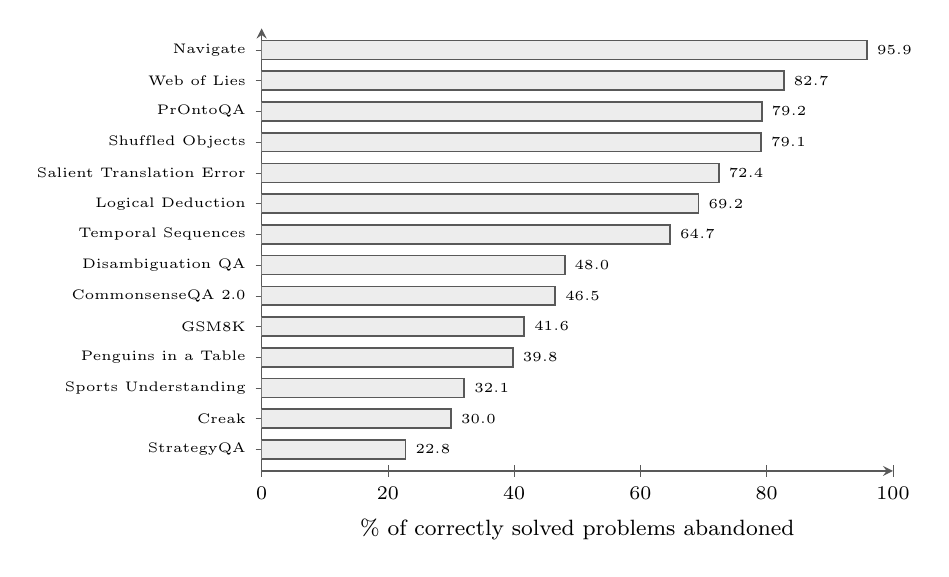
\begin{tikzpicture}
\begin{axis}[width=96mm, height=72mm, xbar, bar width=2.4mm, xmin=0, xmax=100, axis lines=left,
  ymin=0.3, ymax=14.7, ytick={1,...,14}, yticklabels={StrategyQA,Creak,Sports Understanding,Penguins in a Table,GSM8K,CommonsenseQA 2.0,Disambiguation QA,Temporal Sequences,Logical Deduction,Salient Translation Error,Shuffled Objects,PrOntoQA,Web of Lies,Navigate},
  y tick label style={font=\tiny}, xlabel={\% of correctly solved problems abandoned}, nodes near coords, every node near coord/.append style={font=\tiny, /pgf/number format/fixed, /pgf/number format/precision=1, /pgf/number format/fixed zerofill}]
  \addplot[fill=soft, draw=line] coordinates {(22.8,1) (30.0,2) (32.1,3) (39.8,4) (41.6,5) (46.5,6) (48.0,7) (64.7,8) (69.2,9) (72.4,10) (79.1,11) (79.2,12) (82.7,13) (95.9,14)};
\end{axis}
\end{tikzpicture}}

% ---- Article 14: tools and claims ------------------------------------------------------------
\newcommand{\FigToolsClaims}{%
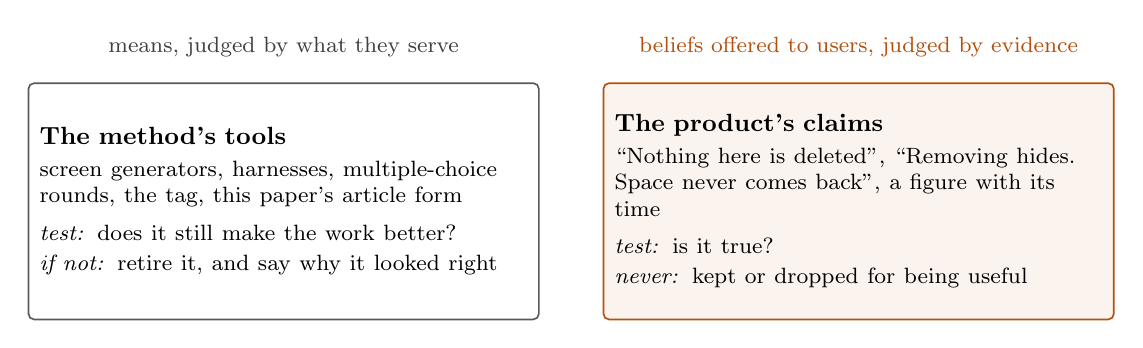
\begin{tikzpicture}
  \node[box, text width=62mm, minimum height=30mm, align=left] (t) {\textbf{The method's tools}\\[2pt]\footnotesize screen generators, harnesses, multiple-choice rounds, the tag, this paper's article form\\[4pt]\textit{test:} does it still make the work better?\\\textit{if not:} retire it, and say why it looked right};
  \node[hot, text width=62mm, minimum height=30mm, align=left, right=8mm of t] (c) {\textbf{The product's claims}\\[2pt]\footnotesize ``Nothing here is deleted'', ``Removing hides. Space never comes back'', a figure with its time\\[4pt]\textit{test:} is it true?\\\textit{never:} kept or dropped for being useful};
  \node[note, above=2mm of t] {means, judged by what they serve};
  \node[note, above=2mm of c, text=accent] {beliefs offered to users, judged by evidence};
\end{tikzpicture}}

% Article 14: Arkes & Blumer (1985), Experiment 3.
\newcommand{\ChartArkes}{%
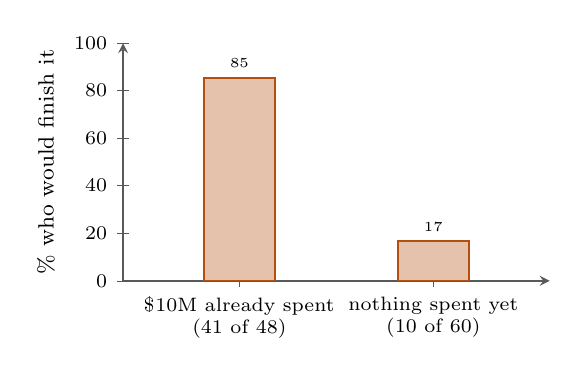
\begin{tikzpicture}
\begin{axis}[width=70mm, height=46mm, ybar, bar width=9mm, ymin=0, ymax=100, axis lines=left,
  xmin=0.4, xmax=2.6, xtick={1,2}, xticklabels={\$10M already spent\\(41 of 48),nothing spent yet\\(10 of 60)}, xticklabel style={align=center}, ylabel={\% who would finish it},
  nodes near coords, every node near coord/.append style={font=\tiny, /pgf/number format/fixed, /pgf/number format/precision=0}]
  \addplot[fill=accent!35, draw=accent] coordinates {(1,85.4) (2,16.7)};
\end{axis}
\end{tikzpicture}}

% ---- Article 15: the loop and its stopping rule ----------------------------------------------
\newcommand{\FigEquilibrium}{%
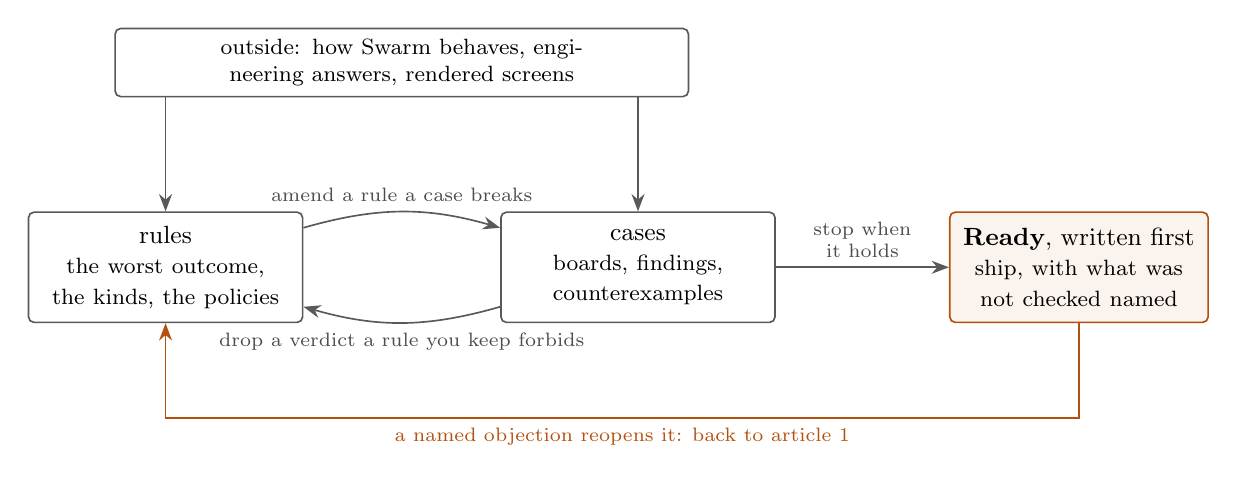
\begin{tikzpicture}
  \node[box, text width=32mm, minimum height=14mm] (p) at (0,0) {rules\\\footnotesize the worst outcome, the kinds, the policies};
  \node[box, text width=32mm, minimum height=14mm] (k) at (60mm,0) {cases\\\footnotesize boards, findings, counterexamples};
  \draw[flow, bend left=16] (p) to node[above, tiny]{amend a rule a case breaks} (k);
  \draw[flow, bend left=16] (k) to node[below, tiny]{drop a verdict a rule you keep forbids} (p);
  \node[box, text width=70mm, font=\footnotesize, minimum height=8mm] (o) at (30mm,26mm) {outside: how Swarm behaves, engineering answers, rendered screens};
  \draw[flow] (o.south -| p.north) -- (p.north); \draw[flow] (o.south -| k.north) -- (k.north);
  \node[hot, text width=30mm, minimum height=14mm] (r) at (116mm,0) {\textbf{Ready}, written first\\\footnotesize ship, with what was not checked named};
  \draw[flow] (k.east) -- node[above, tiny, text width=14mm]{stop when it holds} (r.west);
  \draw[->, accent] (r.south) -- ++(0,-12mm) -| node[pos=0.25, below, tiny, text=accent]{a named objection reopens it: back to article 1} (p.south);
\end{tikzpicture}}
